\documentclass{beamer}

\usepackage{framed}
\usepackage{graphicx}

\begin{document}

\section{Visualizing the distribution of a dataset}
%===========================================================%
\begin{frame}
	\Large
	\noindent \textbf{Visualizing the distribution of a dataset}
	\begin{itemize}
\item When dealing with a set of data, often the first thing you’ll want to do is get a sense for how the variables are distributed.
\item  This chapter of the tutorial will give a brief introduction to some of the tools in seaborn for examining univariate and bivariate distributions. 
\item You may also want to look at the categorical plots chapter for examples of functions that make it easy to compare the distribution of a variable across levels of other variables.
	\end{itemize}

\end{frame}
%=============================================================%
\begin{frame}[fragile]
\Large\begin{framed}
\begin{verbatim}
%matplotlib inline
import numpy as np
import pandas as pd
from scipy import stats, integrate
import matplotlib.pyplot as plt
import seaborn as sns
sns.set(color_codes=True)
np.random.seed(sum(map(ord, 
      "distributions")))
\end{verbatim}
\end{framed}
\end{frame}
%=============================================================%
\section{Plotting univariate distributions}
\begin{frame}[fragile]
The most convenient way to take a quick look at a univariate distribution in seaborn is the distplot() function. By default, this will draw a histogram and fit a kernel density estimate (KDE).

\begin{verbatim}
x = np.random.normal(size=100)
sns.distplot(x);
\end{verbatim}

\begin{figure}
	\centering
	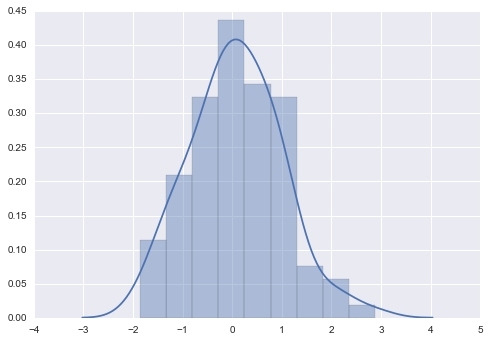
\includegraphics[width=0.7\linewidth]{images/distributions_8_0}
	\caption{}
	\label{fig:distributions_8_0}
\end{figure}

\end{frame}
\section{Histogram}
%===========================================================%
\begin{frame}[fragile]
	\frametitle{Seaborn Workshop}
	\Large
\noindent \textbf{Histograms}
\begin{itemize}
\item Histograms are likely familiar, and a \texttt{hist} function already exists in matplotlib. 
\item A histogram represents the distribution of data by forming bins along the range of the data and then drawing bars to show the number of observations that fall in each bin.
\end{itemize}

\end{frame}
%===========================================================%
\begin{frame}[fragile]
	\frametitle{Seaborn Workshop}
	\large
\begin{itemize}
\item To illustrate this, let’s remove the density curve and add a rug plot, which draws a small vertical tick at each observation. 
\item You can make the rug plot itself with the rugplot() function, but it is also available in \texttt{distplot()}:
\end{itemize}


sns.distplot(x, kde=False, rug=True);
\begin{figure}
\centering
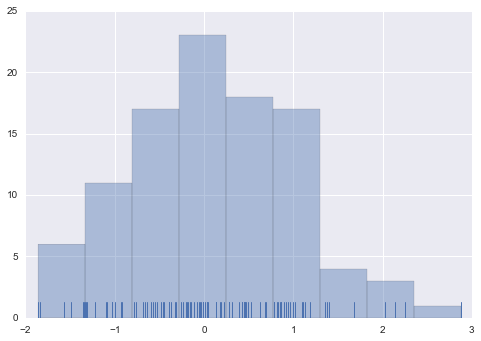
\includegraphics[width=0.7\linewidth]{images/distributions_10_0}
\end{figure}

\end{frame}
%===========================================================%
\begin{frame}[fragile]
	\frametitle{Seaborn Workshop}
	\large
	\begin{itemize}
\item When drawing histograms, the main choice you have is the number of bins to use and where to place them.
\item  \texttt{distplot()} uses a simple rule to make a good guess for what the right number is by default, but trying more or fewer bins might reveal other features in the data:
	\end{itemize}


\end{frame}
%===========================================================%
\begin{frame}[fragile]
		\frametitle{Seaborn Workshop}
		\large
\begin{verbatim}
sns.distplot(x, bins=20, kde=False, rug=True);
\end{verbatim}

\begin{figure}
	\centering
	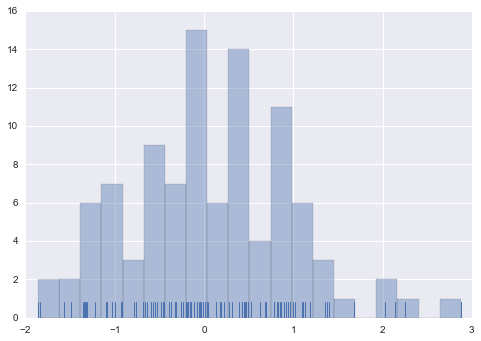
\includegraphics[width=0.7\linewidth]{images/distributions_12_0}
\end{figure}
\end{frame}

%=============================================================%
\section{Kernel density estimaton}
\begin{frame}[fragile]
	\begin{itemize}
		\item The kernel density estimate may be less familiar, but it can be a useful tool for plotting the shape of a distribution. 
		\item Like the histogram, the KDE plots encodes the density of observations on one axis with height along the other axis:
	\end{itemize}	
	
	
	
\end{frame}
%============================================================%
\begin{frame}[fragile]
	\large
	\begin{verbatim}
	
	sns.distplot(x, hist=False, rug=True);
	\end{verbatim}
	\begin{figure}
		\centering
		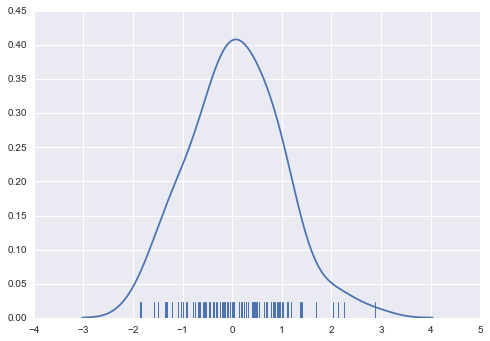
\includegraphics[width=0.7\linewidth]{images/distributions_14_0}
	\end{figure}
\end{frame}
%============================================================%
\begin{frame}[fragile]
	\begin{itemize}
		\item Drawing a KDE is more computationally involved than drawing a histogram.
		\item What happens is that each observation is first replaced with a normal (Gaussian) curve centered at that value:
	\end{itemize}
	
	
\end{frame}
%========================================================== %
\begin{frame}[fragile]
	\begin{framed}
		\begin{verbatim}
		
		x = np.random.normal(0, 1, size=30)
		bandwidth = 1.06 * x.std() * x.size ** (-1 / 5.)
		support = np.linspace(-4, 4, 200)
		
		kernels = []
		for x_i in x:
		
		kernel = stats.norm(x_i, bandwidth).pdf(support)
		kernels.append(kernel)
		plt.plot(support, kernel, color="r")
		
		\end{verbatim}
	\end{framed}
\end{frame}
%=============================================================%
\begin{frame}[fragile]
	\frametitle{Seaborn Workshop}
	\large
	\begin{verbatim}
	sns.rugplot(x, color=".2", linewidth=3);
	\end{verbatim}
	\begin{figure}
		\centering
		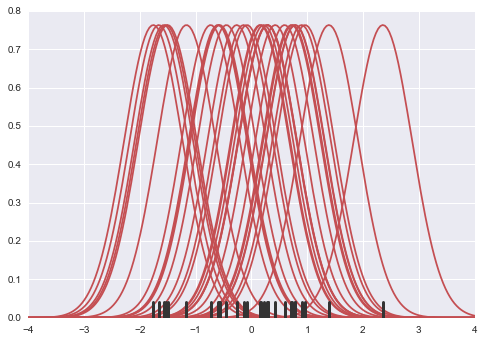
\includegraphics[width=0.7\linewidth]{images/distributions_16_0}
	\end{figure}
	Next, these curves are summed to compute the value of the density at each point in the support grid. The resulting curve is then normalized so that the area under it is equal to 1:
	
\end{frame}
%===========================================================%
\begin{frame}[fragile]
	\frametitle{Seaborn Workshop}
	\large
	\begin{verbatim}
	density = np.sum(kernels, axis=0)
	density /= integrate.trapz(density, support)
	plt.plot(support, density);
	\end{verbatim}
	
	\begin{figure}
		\centering
		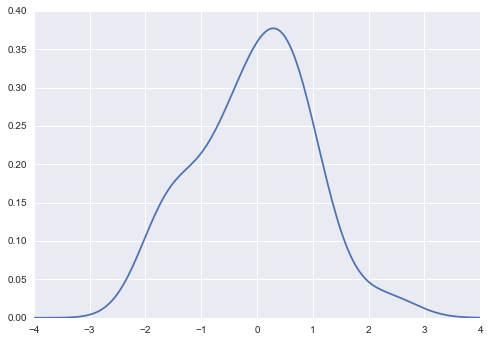
\includegraphics[width=0.7\linewidth]{images/distributions_18_0}
	\end{figure}
\end{frame}
%===========================================================%
\begin{frame}[fragile]
	
	\frametitle{Seaborn Workshop}
	\large
	\begin{itemize}
		\item We can see that if we use the \texttt{kdeplot()} function in seaborn, we get the same curve. 
		\item This function is used by \texttt{distplot()}, but it provides a more direct interface with easier access to other options when you just want the density estimate:
	\end{itemize}
	
	
\end{frame}
%=============================================== %
\begin{frame}[fragile]
	\frametitle{Seaborn Workshop}
	\large
	\begin{framed}
		\begin{verbatim}
		sns.kdeplot(x, shade=True);
		\end{verbatim}
	\end{framed}
	
	\begin{figure}
		\centering
		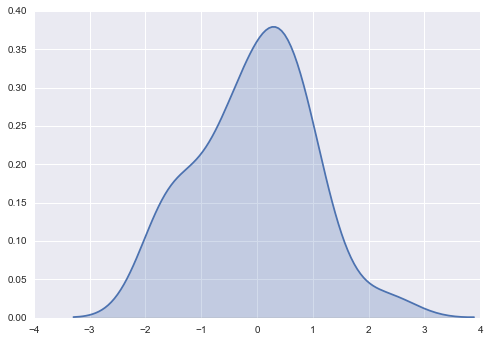
\includegraphics[width=0.7\linewidth]{images/distributions_20_0}
	\end{figure}
	
\end{frame}
%=============================================== %
\begin{frame}[fragile]
	\frametitle{Seaborn Workshop}
	\large
	\begin{itemize}
		\item The bandwidth (\texttt{bw}) parameter of the KDE controls how tightly the estimation is fit to the data, much like the bin size in a histogram. 
		\item It corresponds to the width of the kernels we plotted above. \item The default behavior tries to guess a good value using a common reference rule, but it may be helpful to try larger or smaller values:
	\end{itemize}
	
	
\end{frame}
%===========================================================%
\begin{frame}[fragile]
	\frametitle{Seaborn Workshop}
	\large
	\begin{verbatim}
	{sns.kdeplot(x)
	sns.kdeplot(x, bw=.2, label="bw: 0.2")
	sns.kdeplot(x, bw=2, label="bw: 2")
	plt.legend();...}
	\end{verbatim}
	
	\begin{figure}
		\centering
		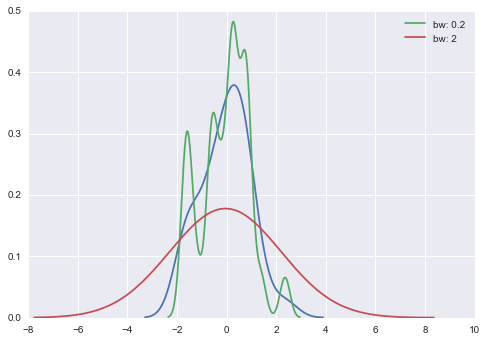
\includegraphics[width=0.7\linewidth]{images/distributions_22_0}
	\end{figure}
	
\end{frame}
%===========================================================%
\begin{frame}[fragile]
	\frametitle{Seaborn Workshop}
	\large
	\begin{itemize}
		\item As you can see above, the nature of the Gaussian KDE process means that estimation extends past the largest and smallest values in the dataset. 
		\item It’s possible to control how far past the extreme values the curve is drawn with the cut parameter; however, this only influences how the curve is drawn and not how it is fit:
	\end{itemize}
\end{frame}
%============================================================%
\begin{frame}[fragile]
	\frametitle{Seaborn Workshop}
	\begin{verbatim}
	sns.kdeplot(x, shade=True, cut=0)
	sns.rugplot(x);
	\end{verbatim}
	
	\begin{figure}
		\centering
		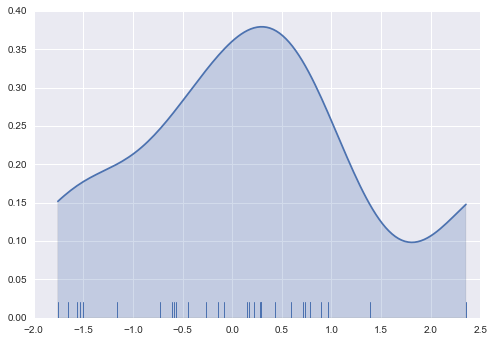
\includegraphics[width=0.7\linewidth]{images/distributions_24_0}
	\end{figure}
\end{frame}
\section{Fitting parametric distributions}
%============================================================%
\begin{frame}[fragile]
	\frametitle{Seaborn Workshop}\large
	\noindent \textbf{Fitting parametric distributions}\\
	You can also use \texttt{distplot()} to fit a parametric distribution to a dataset and visually evaluate how closely it corresponds to the observed data:
	
\end{frame}
%============================================================%
\begin{frame}[fragile]
	\frametitle{Seaborn Workshop}
	\begin{framed}
		\begin{verbatim}
		x = np.random.gamma(6, size=200)
		sns.distplot(x, kde=False, fit=stats.gamma);
		\end{verbatim}
	\end{framed}
	
	\begin{figure}
		\centering
		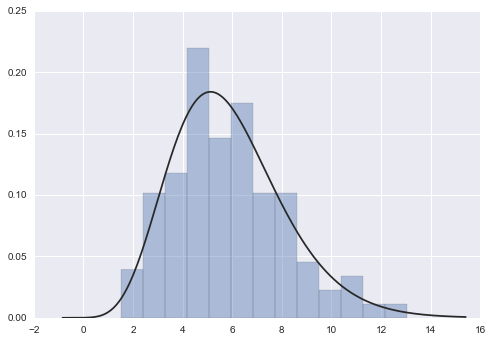
\includegraphics[width=0.7\linewidth]{images/distributions_26_0}
		\caption{}
		\label{fig:distributions_26_0}
	\end{figure}
\end{frame}


\section{Plotting Bivariate Bistributions}
\begin{frame}[fragile]
	\large
	\noindent \textbf{Plotting Bivariate Bistributions}
	
	\begin{itemize}
		\item It can also be useful to visualize a bivariate distribution of two variables. 
		\item The easiest way to do this in seaborn is to just the \texttt{jointplot()} function, which creates a multi-panel figure that shows both the bivariate (or joint) relationship between two variables along with the univariate (or marginal) distribution of each on separate axes.
	\end{itemize}
	
	
\end{frame}
%==============================================================%

\begin{frame}[fragile]
	\frametitle{Seaborn Workshop}
	\large
	\begin{framed}
		\begin{verbatim}
		mean, cov = [0, 1], [(1, .5), (.5, 1)]
		
		data = np.random.multivariate_normal(mean, 
		cov, 200)
		
		df = pd.DataFrame(data, columns=["x", "y"])
		\end{verbatim}
	\end{framed}
	
\end{frame}
%==============================================================%
\section{Scatterplots}
\begin{frame}[fragile]
	\large
	\begin{itemize}
		\item The most familiar way to visualize a bivariate distribution is a scatterplot, where each observation is shown with point at the x and y values. 
		\item This is analgous to a rug plot on two dimensions. 
		\item You can draw a scatterplot with the matplotlib \texttt{plt.scatter} function, and it is also the default kind of plot shown by the \texttt{jointplot()} function:
	\end{itemize}
	
	
\end{frame}

%===========================================================%
\begin{frame}[fragile]
	\frametitle{Seaborn Workshop}
	\large
	\begin{framed}
		\begin{verbatim}
		sns.jointplot(x="x", y="y", data=df);
		\end{verbatim}
	\end{framed}
	\begin{figure}
		\centering
		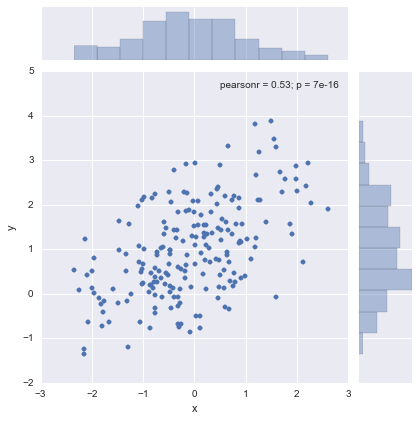
\includegraphics[width=0.55\linewidth]{images/distributions_30_0}
	\end{figure}
	
\end{frame}
\section{Hexbin Plots}
%===========================================================%
\begin{frame}[fragile]
	\large
	\noindent \textbf{Hexbin plots}
	\begin{itemize}
		\item The bivariate analogue of a histogram is known as a “hexbin” plot, because it shows the counts of observations that fall within hexagonal bins. \item This plot works best with relatively large datasets. 
		\item It’s availible through the matplotlib \texttt{plt.hexbin} function and as a style in \texttt{jointplot()}. 
		\item It looks best with a white background:
	\end{itemize}
	
\end{frame}
%===========================================================%
\begin{frame}[fragile]
	\begin{verbatim}
	x, y = np.random.multivariate_normal(mean, cov, 1000).T
	with sns.axes_style("white"):
	sns.jointplot(x=x, y=y, kind="hex", color="k");
	\end{verbatim}
	
	\begin{figure}
		\centering
		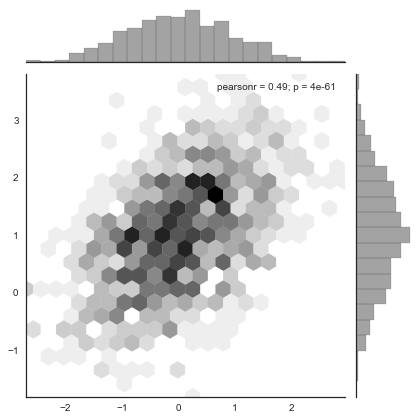
\includegraphics[width=0.7\linewidth]{images/distributions_32_0}
		
	\end{figure}
	
\end{frame}
%===========================================================%
\begin{frame}[fragile]
	\frametitle{Kernel density estimation}
	\large
	\begin{itemize}
		\item It is also posible to use the kernel density estimation procedure described above to visualize a bivariate distribution. 
		\item In seaborn, this kind of plot is shown with a contour plot and is available as a style in \texttt{jointplot()}:
	\end{itemize}
	
\end{frame}
%===========================================================%
\begin{frame}[fragile]
	\frametitle{Seaborn Workshop}
	\large
	\begin{framed}
		\begin{verbatim}
		sns.jointplot(x="x", y="y", data=df, kind="kde");
		\end{verbatim}
	\end{framed}
	\begin{figure}
		\centering
		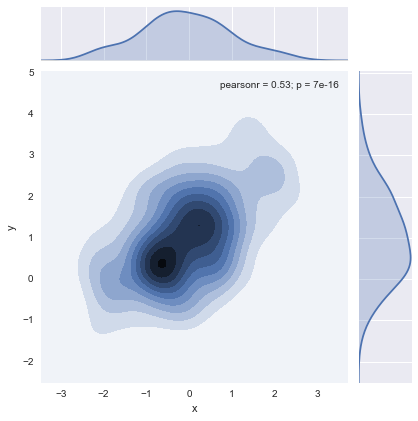
\includegraphics[width=0.55\linewidth]{images/distributions_34_0}
	\end{figure}
\end{frame}
%===========================================================%
\begin{frame}[fragile]
	\frametitle{Seaborn Workshop}
	\large
	\begin{itemize}
		\item You can also draw a two-dimensional kernel density plot with the \texttt{kdeplot()} function.
		\item  This allows you to draw this kind of plot onto a specific (and possibly already existing) matplotlib axes, whereas the \texttt{jointplot()} function manages its own figure:
	\end{itemize}
\end{frame}
%===========================================================%
\begin{frame}[fragile]
	\begin{framed}
		\begin{verbatim}
		f, ax = plt.subplots(figsize=(6, 6))
		sns.kdeplot(df.x, df.y, ax=ax)
		sns.rugplot(df.x, color="g", ax=ax)
		sns.rugplot(df.y, vertical=True, ax=ax);
		\end{verbatim}
	\end{framed}
	\begin{figure}
		\centering
		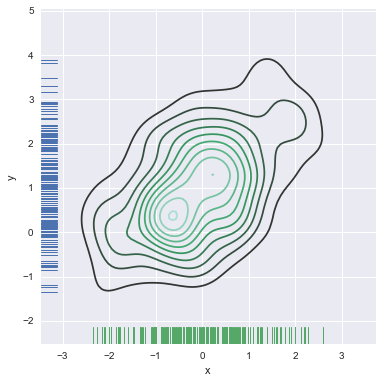
\includegraphics[width=0.55\linewidth]{images/distributions_36_0}
	\end{figure}
	
\end{frame}
%===========================================================%
\begin{frame}[fragile]
	\large
	If you wish to show the bivariate density more continuously, you can simply increase the number of contour levels:
	\begin{verbatim}
	f, ax = plt.subplots(figsize=(6, 6))
	cmap = sns.cubehelix_palette(as_cmap=True, dark=0, light=1, reverse=True)
	sns.kdeplot(df.x, df.y, cmap=cmap, n_levels=60, shade=True);
	\end{verbatim}
\end{frame}
%===========================================================%
\begin{frame}[fragile]
	\frametitle{Hexbin Plots}
	\large
	\begin{figure}
		\centering
		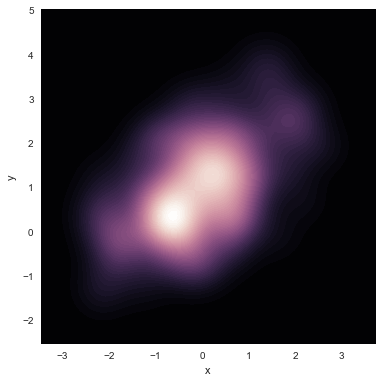
\includegraphics[width=0.55\linewidth]{images/distributions_38_0}
	\end{figure}
	
	
\end{frame}
%===========================================================%
\begin{frame}[fragile]
	\frametitle{Seaborn Workshop}
	\large
	\begin{itemize}
		\item The \texttt{jointplot()} function uses a \texttt{JointGrid} to manage the figure. \bigskip
		\item For more flexibility, you may want to draw your figure by using \texttt{JointGrid} directly. \bigskip
		\item  \texttt{jointplot()} returns the \texttt{JointGrid} object after plotting, which you can use to add more layers or to tweak other aspects of the visualization:
	\end{itemize}
	
	
	
	
\end{frame}
%===========================================================%
\begin{frame}[fragile]
	\frametitle{Seaborn Workshop}	\large
	
	\begin{framed}
		\begin{verbatim}
		g = sns.jointplot(x="x", y="y", 
		data=df, kind="kde", color="m")
		
		g.plot_joint(plt.scatter, c="w", 
		s=30, linewidth=1, marker="+")
		
		g.ax_joint.collections[0].set_alpha(0)
		
		g.set_axis_labels("$X$", "$Y$");
		\end{verbatim}
	\end{framed}
\end{frame}
%===========================================================%
\begin{frame}[fragile]
	\large
	\begin{figure}
		\centering
		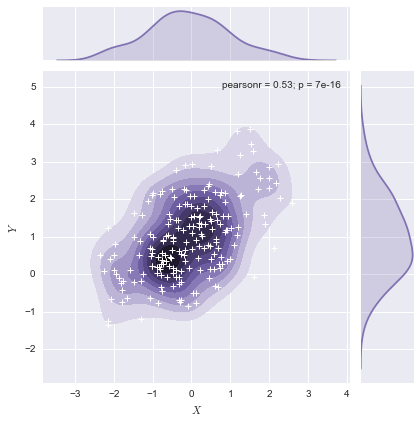
\includegraphics[width=0.75\linewidth]{images/distributions_40_0}
	\end{figure}
	
	
\end{frame}

\section{Visualizing pairwise relationships in a dataset}
%===========================================================%
\begin{frame}[fragile]
	\Large
	\begin{itemize}
		\item To plot multiple pairwise bivariate distributions in a dataset, you can use the \texttt{pairplot()} function.
		\item  This creates a matrix of axes and shows the relationship for each pair of columns in a DataFrame. 
		\item By default, it also draws the univariate distribution of each variable on the diagonal Axes:
	\end{itemize}
	\begin{verbatim}
	iris = sns.load_dataset("iris")
	sns.pairplot(iris);
	\end{verbatim}
\end{frame}
%===========================================================%
\begin{frame}
	\begin{figure}
		\centering
		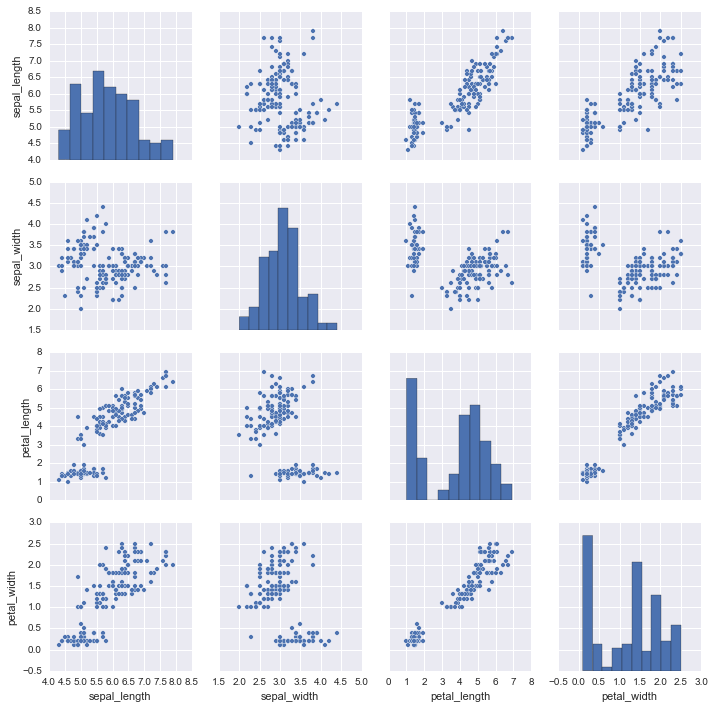
\includegraphics[width=0.8\linewidth]{images/distributions_42_0}
		\caption{}
		\label{fig:distributions_42_0}
	\end{figure}
	
\end{frame}
%===========================================================%
\begin{frame}[fragile]
	\frametitle{Seaborn Workshop}
	\large
	Much like the relationship between \texttt{jointplot()} and \texttt{JointGrid}, the \texttt{pairplot()} function is built on top of a \texttt{PairGrid} object, which can be used directly for more flexibility:
	\begin{framed}
		\begin{verbatim}
		g = sns.PairGrid(iris)
		g.map_diag(sns.kdeplot)
		g.map_offdiag(sns.kdeplot, cmap="Blues_d", 
		n_levels=6);
		\end{verbatim}
	\end{framed}
\end{frame}
%========================================================= %
%/Users/mwaskom/anaconda/lib/python2.7/site-packages/matplotlib/axes/_axes.py:475: UserWarning: No labelled objects found. Use label='...' kwarg on individual plots.
%  warnings.warn("No labelled objects found. "
%../_images/distributions_44_1.png
\begin{frame}[fragile]
	\begin{figure}
		\centering
		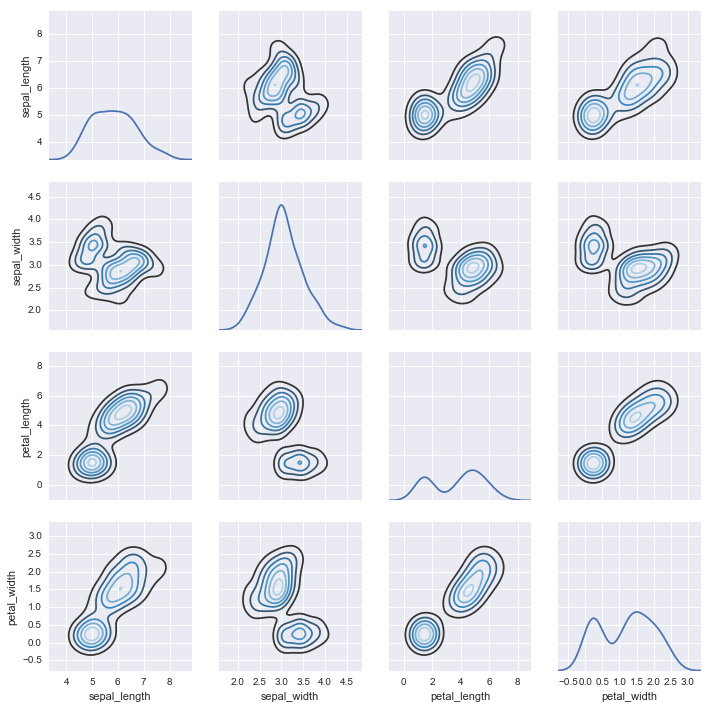
\includegraphics[width=0.7\linewidth]{images/distributions_44_1}
	\end{figure}
\end{frame}
\end{document}
